% vim:ft=tex:
%
\documentclass[12pt]{article}
\usepackage{hyperref}
\usepackage{graphicx}
\usepackage{amsmath}
\title{progress
}
\author{gareths --- \texttt{gareths@mds041-OptiPlex-780}}

\begin{document}
\maketitle
\pagebreak
Hi Brett and Steve.\\\\
This is the progress I have made so far with estimating parameters using metropolis hastings. I have coded both a standard metropolis hastings into Matlab and c. I have then coded a simulated Annealing algorithm into Matlab. The simulated annealing algorithm as far as I can tell is more successful than the standard metropolis hastings. I have had to play around a bit with how to test the closeness of fit for the likelihood functions in the algorithms. I will hopeful explain my reasoning alright for each one. The next step I think is to take the Simulated annealing algorithm to an MPI code and then to GPU. \\

The MPI code will simply allow a comparison between a serial algorithm on a CPU to a multi-threaded implementation. To do this I don't think will be too difficult. Just for each temperature we send out multiple seed values and only take the best one for the next temperature iteration. I also want to take the standard metropolis to multi-thread for comparison. Since the two algorithms are extremely similar it would just be nice for comparison.\\

A concern for me is the estimation for the noise in the system. When I attempt to add noise to the output and try to fit a noise parameter to the output of the model filter I get a small value with the other parameters seemingly averaging out the noisy output. I'll include an image for what I mean here.\\

I've kept all of my code updated on github. If you want to compile and run the c code you'll need the gnu scientific library (gsl) for the random number generations. The matlab code for my metropolis hastings and simulated annealing is also on there. The metropolis hastings algorithm is in the \textbf{butterworth} folder. \url{https://github.com/sciff90?tab=repositories}

\section{Standard Metropolis Hastings}
To code this one up I have used basically a step response to a nth order IIR filter. The frequency response of which I can play around with. This is largely unimportant however. The results for the lower order filters are promising with the first order filter being fit reasonably well i.e the residual error is of the order of $10^{-5}$. However when applying this to higher order filters with more unknowns I am getting at least for a single mcmc chain what appears to be multimodal solutions corrupting each other rather than distinct peaks for each unknown parameter. I believe this is due to the algorithm getting stuck in local minimums of the error function. This was the main reason I went to a simulated annealing algorithm. I still plan to fully parallelize this algorithm for comparison between algorithms as in essence these algorithm are all very similar. My assumption for the output of a metropolis hastings algorithm is that we should get a gaussian distributed answer who's mean is close to the real value of the parameter. If this is the case even the first order mean is not entirely centred around the expected values. I keep a track of the best solution (least error) and this is usually very close to what is expected.
\subsection{Residual error function $\epsilon$}
Initially I was having difficulty with the error function for testing the closeness of the fit of the parameters. I have ended up using the sum of the residual square errors. This however wasn't enough in the tests I did so I expanded to have multiple input function (a combination of steps and trig functions) to try and prevent lots of possible minimisations being picked up by the algorithm.\\
The input vector $\mathbf{u} = [u_1 u_2 u_3.....u_n]$ has output response $\mathbf{y} = [y_1 y_2 y_3.....y_n]$. This for the most part helped greatly with local minima at least for the lower order filters. The problem still remains as the order of the filter increases. In order to have a single number to represent the overall error of multiple input functions I have taken the norm(2) error of the individual errors. The filter is assumed to be correct if this error $\epsilon < 10^{-5}$.

$$\epsilon = \sqrt{\left[\sum^{n-1}_{j = 0}{\sum^{N-1}_{k=0} \left(y_{out}[k]-y_{mdl}[k]\right)^2}}\right]^2$$
where,\\
$N$ is the number of samples\\
$n$ is the number of input functions used\\
$y_{out}$ is the known output\\
$y_{mdl}$ is the model output\\
$\epsilon$ is the error in the fit

This error function is used to generate the acceptance test for the ``accept or reject" step. This is basically the ratio of the current error function $\epsilon_{curr}$ with the candidate error function $\epsilon_{cand}$. These have to be turned in probability density functions however which we choose as Gaussian. Therefore the overall probability to test is:

$$\alpha = exp\left(-\epsilon_{cand}+\epsilon_{curr}\right)$$
If the candidate function is better this will lead to a value $> 0$ and therefore the exponential of this will be greater than 1. The candidate is accepted if $\alpha > rand[0,1]$. This means that sometimes even though the candidate may be a worse fit it is still accepted.

\\
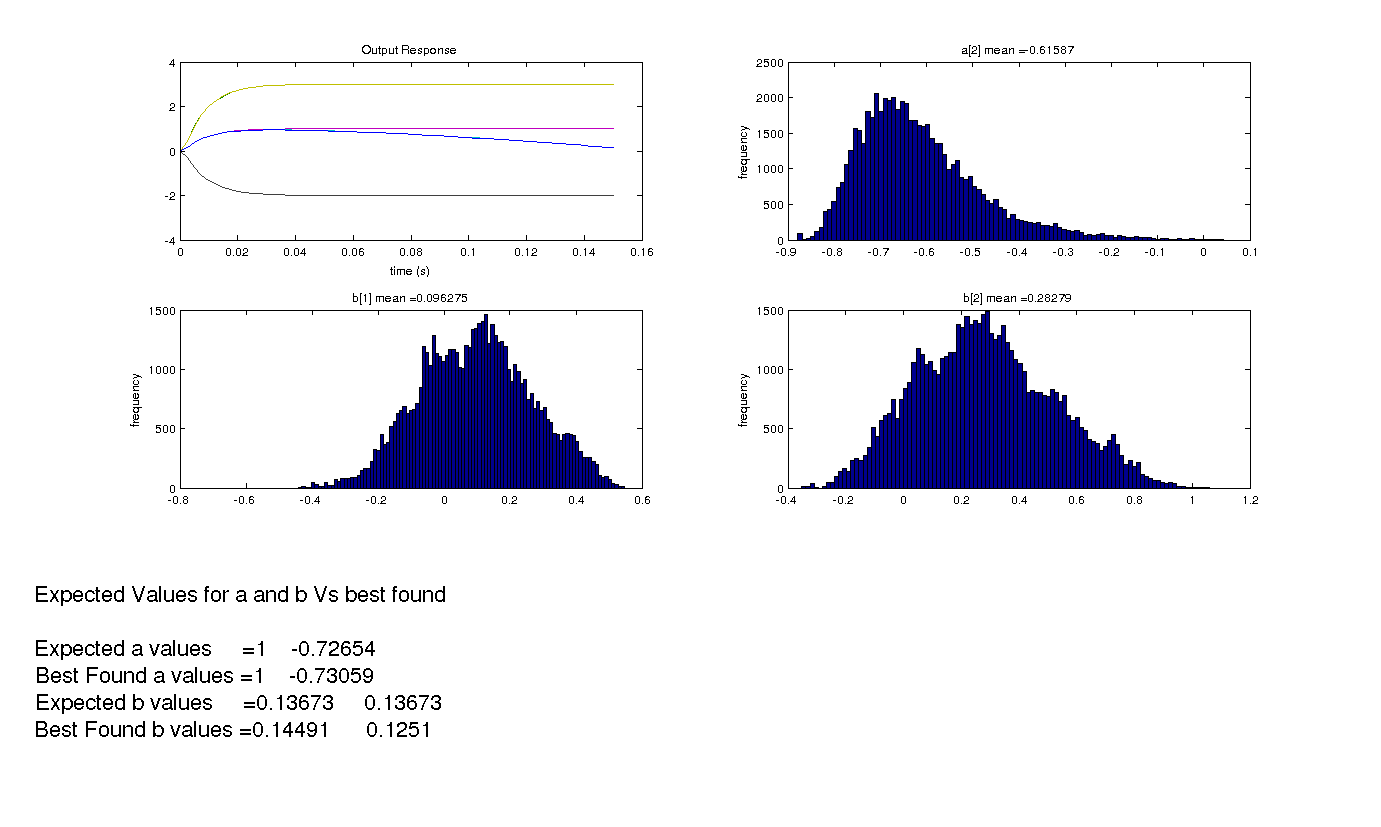
\includegraphics[width=\linewidth]{./plots/met_hast_order1.png}

\section{Simulated Annealing }
The next step I went to was to use a simulated annealing algorithm. This as far as my understanding goes slowly restrict the domain over which the likelihood function is accepted. You run a number of random seeds for each ``temperature " iteration and then take the best one as you slowly cool the system. The main difference is the acceptance probability function which instead of being:
$$\alpha = min(rand[0,1],1)$$
it is instead 
$$\alpha = min(rand[0,1],e^{-\frac{\Delta y}{T}})$$
\\\\where $\Delta y$ is the error function $\epsilon_{curr} -\epsilon_{cand}$ and $T$ is the current ``Temperature". This means that if the candidate error is less than the current error it is always accepted. However if it is not it is accepted based on the current ``temperature" and the $\Delta Y$. As the algorithm progresses the likelihood of accepting a move that isn't better than the current values is decreased. Meaning that once an area of high probability is reached it is much more difficult for the algorithm to accept moves away from this high probability region. As long as the system is cooled ``sufficiently slowly this will find a global minimum, thus minimising the error function and finding the correct parameters.\\

The problem however is that ``sufficiently slowly" is a logarithmic relationship. This algorithm does indeed work very well for a second and even third order systems but a uniform stepsize and cooling schedule is the algorithms downfall. The cooling schedule I am using is a geometric one:
$$T = T \times T_{change}$$
and the neighbour move is a normal distributed move with and standard deviation $\sigma = 0.01$ for these test filters. With this cooling schedule having initial temperature $T_{max} = 100000$ and $T_{change} = 0.9999$ the algorithm works rather well for 2nd order systems and depending on the initial acceptances sometimes 3rd order. It is also far quicker in finding a very accurate solution than the standard metropolis hastings. To make this algorithm parallel should also be relatively simple as it comprises two loops.\\

The outer loop controls the cooling rate and th inner loop distributes K random samples for each temperature. This inner loop could be put onto a GPU relatively easily as we would just send of K random seeds and take the best random value found for each temperature. This is the next step for this algorithm. I was however going to try an adaptive simulated annealing algorithm as well. This has the ability to change stepsize and the cooling rate as the algorithm progresses. The ability to change stepsize is important as when we get very close to a solution if the movements are too big none will be accepted especially if the algorithm is a long way into the cooling period.
\\

Again the code for these algorithms are on github at \url{https://github.com/sciff90?tab=repositories} if you wish to run them and let me know if they make sense to you. I think the next step is to try the adaptive simulated annealing based on this paper \url{http://www.sciencedirect.com/science/article/pii/S1051200400903841}. This is where I am pretty much up to as of 26/8.

Thanks Gareth


\end{document}
